%%%%%%%%%%%%%%%%%%%%%%%%%%%%%%%%%%%%%%%%%%%%%%%%%%%%%%%%%%%%%%%%%%%%%%%%%%%%%%%%
% Preambles
%%%%%%%%%%%%%%%%%%%%%%%%%%%%%%%%%%%%%%%%%%%%%%%%%%%%%%%%%%%%%%%%%%%%%%%%%%%%%%%%
\documentclass[aspectratio=169,xcolor=x11names,table]{beamer}
\mode<presentation>{
	% theme
	\usetheme{Luebeck}
	\hypersetup{pdfpagemode=FullScreen}
		\setbeamertemplate{headline}[default]
	\setbeamertemplate{navigation symbols}{}
	% \setbeamertemplate{caption}[numbered]
		\usefonttheme{professionalfonts}
	% logo
	% \addtobeamertemplate{frametitle}{}{
	% 	\begin{textblock*}{100mm}(0.8\textwidth,-7mm)
	% 		
\includegraphics[height=5mm]{sams.jpg}
	% 	\end{textblock*}
	% }
	% footnote
	\setbeamertemplate{footline}[text line]{%
			\parbox{\linewidth}{\vspace*{-8pt}Tutorial - Time Sereies Analysis\hfill\insertshortauthor\hfill\insertframenumber/\inserttotalframenumber}}

	% transparent cover
	\setbeamercovered{transparent}
}

% define your own colors:
\definecolor{KFUPMgreen}{cmyk}{0.756,0,0.756,0.196}
\definecolor{tech_gold}{RGB}{179,163,105}
\definecolor{buzz_gold}{RGB}{234,170,0}
\definecolor{tech_blue}{RGB}{0,38,58}
\definecolor{sams_dark_blue}{RGB}{0,75,141}
\definecolor{sams_medium_blue}{RGB}{0,105,170}
\definecolor{sams_light_blue}{RGB}{0,129,198}
\definecolor{sams_green}{RGB}{93,151,50}
\setbeamercolor{structure}{fg=sams_dark_blue, bg=white}
\setbeamercolor*{palette primary}{use=structure,fg=white,bg=sams_medium_blue}

%%%%%%%%%%%%%%%%%%%%%%%%%%%%%%%%%%%%%%%%%%%%%%%%%%%%%%%%%%%%%%%%%%%%%%%%%%%%%%%%
% Dependencies
%%%%%%%%%%%%%%%%%%%%%%%%%%%%%%%%%%%%%%%%%%%%%%%%%%%%%%%%%%%%%%%%%%%%%%%%%%%%%%%%
\usepackage[utf8]{inputenc}
\usepackage[english]{babel}
\usepackage[backend=bibtex,
	 sorting=none,
	 maxcitenames=2,
	 mincitenames=1,
	 citestyle=authoryear,
	 maxbibnames=99]{biblatex}
\usepackage{csquotes}
\usepackage{lmodern}    % font at arbitrary size
\usepackage{mathtools}
\usepackage{graphicx}
\graphicspath{{fig/}}
\usepackage{color}
\usepackage{bm}
\usepackage{booktabs}
\usepackage{subcaption}
\usepackage{appendixnumberbeamer}
\usepackage{textpos}
\usepackage{datetime}
\usepackage[linesnumbered,ruled,vlined,slovak]{algorithm2e}
\usepackage{animate}
\usepackage{subcaption}
\usepackage{multirow}

%%%%%%%%%%%%%%%%%%%%%%%%%%%%%%%%%%%%%%%%%%%%%%%%%%%%%%%%%%%%%%%%%%%%%%%%%%%%%%%%
% Bibliography
%%%%%%%%%%%%%%%%%%%%%%%%%%%%%%%%%%%%%%%%%%%%%%%%%%%%%%%%%%%%%%%%%%%%%%%%%%%%%%%%
\bibliography{time_series.bib}

%%%%%%%%%%%%%%%%%%%%%%%%%%%%%%%%%%%%%%%%%%%%%%%%%%%%%%%%%%%%%%%%%%%%%%%%%%%%%%%%
% Title Page
%%%%%%%%%%%%%%%%%%%%%%%%%%%%%%%%%%%%%%%%%%%%%%%%%%%%%%%%%%%%%%%%%%%%%%%%%%%%%%%%
\title{Robust Time Series Analysis and Applications}
\subtitle{An Industry Perspective}
\author[Lijun Zhu]{
	{\Large Lijun Zhu}\\
	\vspace{3mm}
	Senior Manager
}
\institute{Data Science and Engineering, Sam's Club}
\newdate{date}{17}{11}{2022}
\date{\small\displaydate{date}}

%%%%%%%%%%%%%%%%%%%%%%%%%%%%%%%%%%%%%%%%%%%%%%%%%%%%%%%%%%%%%%%%%%%%%%%%%%%%%%%%
%  Outline at each section
%%%%%%%%%%%%%%%%%%%%%%%%%%%%%%%%%%%%%%%%%%%%%%%%%%%%%%%%%%%%%%%%%%%%%%%%%%%%%%%%
\AtBeginSection[] {
    \begin{frame}
        \frametitle{Outline}
        \tableofcontents
        [
            currentsection,
            currentsubsection,
            subsectionstyle=show/show/hide
        ]
        \addtocounter{framenumber}{-1}
    \end{frame}
}

%%%%%%%%%%%%%%%%%%%%%%%%%%%%%%%%%%%%%%%%%%%%%%%%%%%%%%%%%%%%%%%%%%%%%%%%%%%%%%%%
% Content
%%%%%%%%%%%%%%%%%%%%%%%%%%%%%%%%%%%%%%%%%%%%%%%%%%%%%%%%%%%%%%%%%%%%%%%%%%%%%%%%
\begin{document}

% title page
{
	%
	\usebackgroundtemplate{
\includegraphics[width=1\paperwidth]{sams_background}}
	%
	\begin{frame}[noframenumbering,plain]
		% \hfill
		% \begin{minipage}{0.65\paperwidth}
		\titlepage
		% \end{minipage}
	\end{frame}
	\setcounter{framenumber}{0}
}

% introduction
\begin{frame}{Who am I?}
	\begin{columns}
		\begin{column}{0.8\linewidth}
		\begin{itemize}
			\item Lijun Zhu, Ph.D.
				\begin{itemize}
					\item Machine Learning, Data Science, and Signal Processing
					\item Leading a team of 10-20 DS, DE, MLE, and SDE
					\item Previous experience in internship, Co-op, IC, and PM
				\end{itemize}
			\item Sam's Club Data Science and Engineering
				\begin{itemize}
					\item A centralized data science / machine learning group
					\item Full stack data scientists from product concept to production
					\item Impactful product and initiatives spanning all field in data science
						\begin{itemize}
							\item Time series forecast
							\item Optimization
							\item NLP chat bot and text analysis
							\item Fraud detection
						\end{itemize}
				\end{itemize}
			\item Full time and internship opportunities every year
				\begin{itemize}
					\item Organization trippled in size for the past three years
				\end{itemize}
		\end{itemize}
		\end{column}
		\hfill
		\begin{column}{0.2\linewidth}
			\begin{figure}
				\centering
				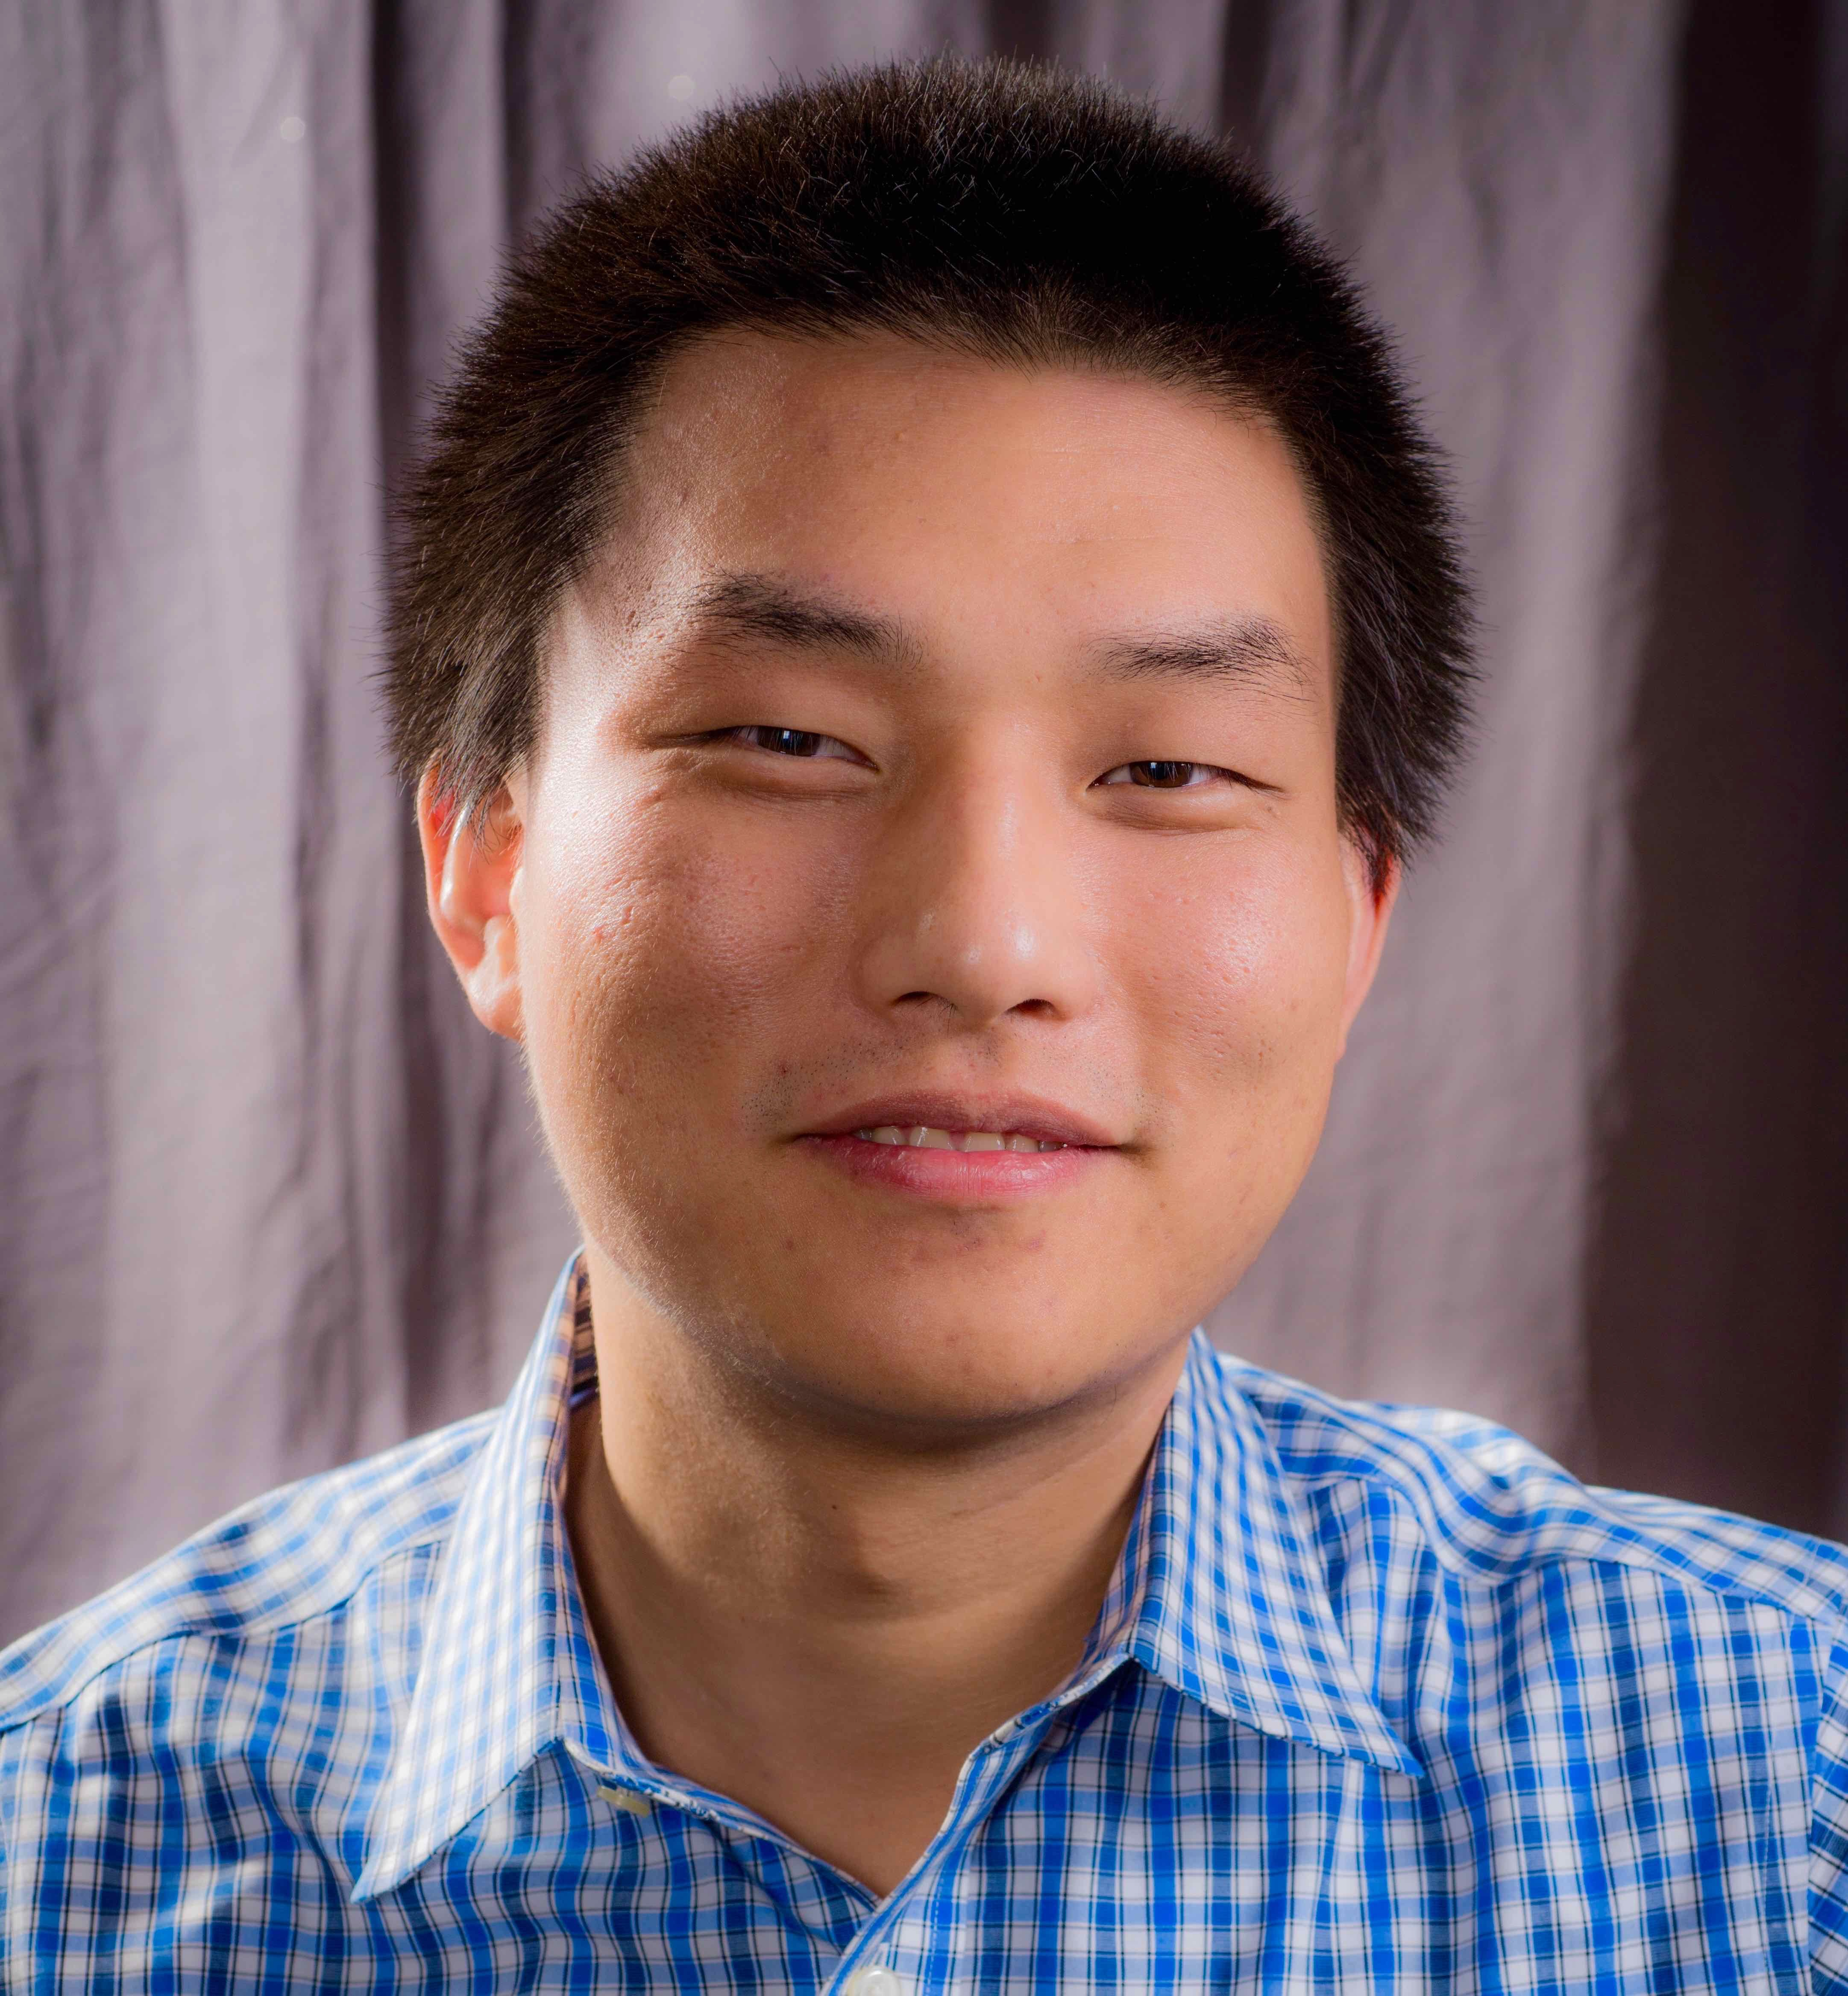
\includegraphics[width=\columnwidth]{lijun}
			\end{figure}
			\vspace{2mm}
			\begin{figure}
				\centering
				
\includegraphics[width=\columnwidth]{sams_logo}
			\end{figure}
		\end{column}
	\end{columns}
\end{frame}

\begin{frame}
	\frametitle{Disclosures}
	\begin{itemize}
		\item Nothing worth learning can be taught
			\begin{itemize}
				\item Not here to teach but to communicate
				\item Interactive session, questions/discussion are welcomed any time
			\end{itemize}
			\vspace{1cm}
		\item Nothing specific about Walmart or Sam's Club will be discussed
			\begin{itemize}
				\item No insider information about the company
				\item No specific data/project/product will be discussed
			\end{itemize}
	\end{itemize}
\end{frame}

\begin{frame}
	\frametitle{Outline}
	\tableofcontents[hideallsubsections]
\end{frame}

%-------------------------------------------------------------------------------
% Time series analysis basics
%-------------------------------------------------------------------------------
\section{Time series analysis}
\subsection{What is time series}
\begin{frame}
	\frametitle{Time Series is Ubiquitous}
	\begin{columns}
		\begin{column}{0.4\linewidth}
			\begin{itemize}
				\item Time series record a history of states
					\begin{itemize}
						\item price hisory
						\item sales records
						\item sensor signal
						\item operational log
					\end{itemize}
				\item History is useful if it helps us make decisions
				\item Decision leads to business impact
			\end{itemize}
		\end{column}
		\hfill
		\begin{column}{0.6\linewidth}
			\begin{figure}
				\centering
				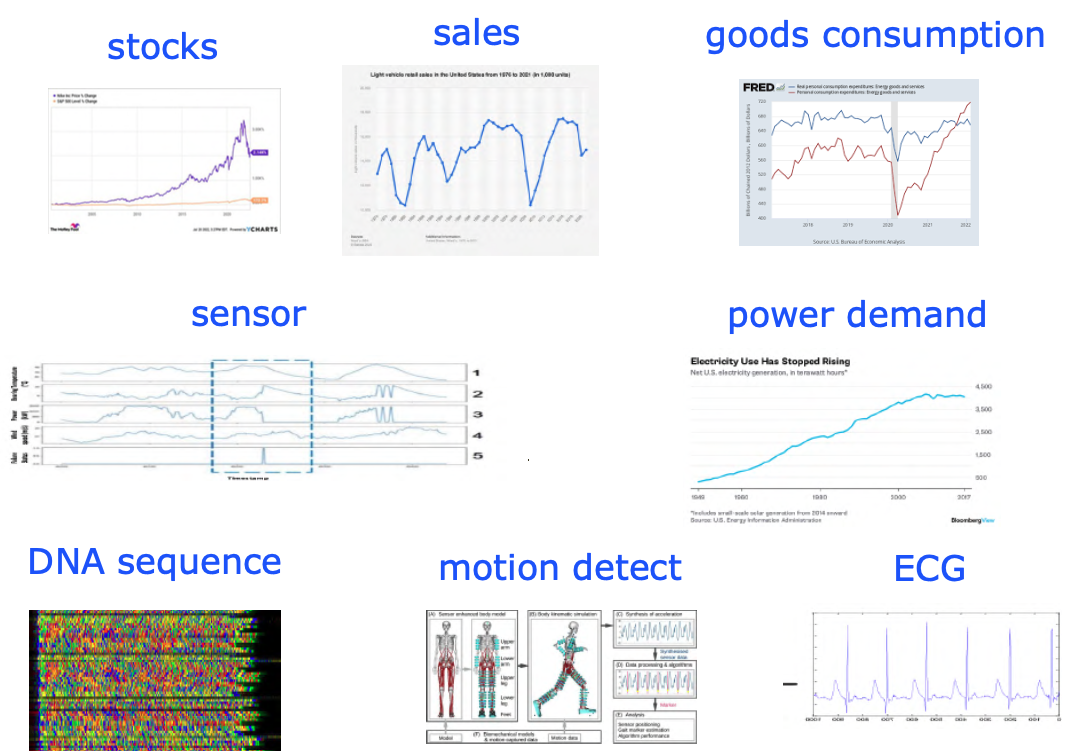
\includegraphics[width=\columnwidth]{time_series}
				\tiny{Image courtesy of \cite{wen2022robust}.}
			\end{figure}
		\end{column}
	\end{columns}
\end{frame}

\begin{frame}
	\frametitle{Typical Applications on Time Series}
	\begin{figure}
		\centering
		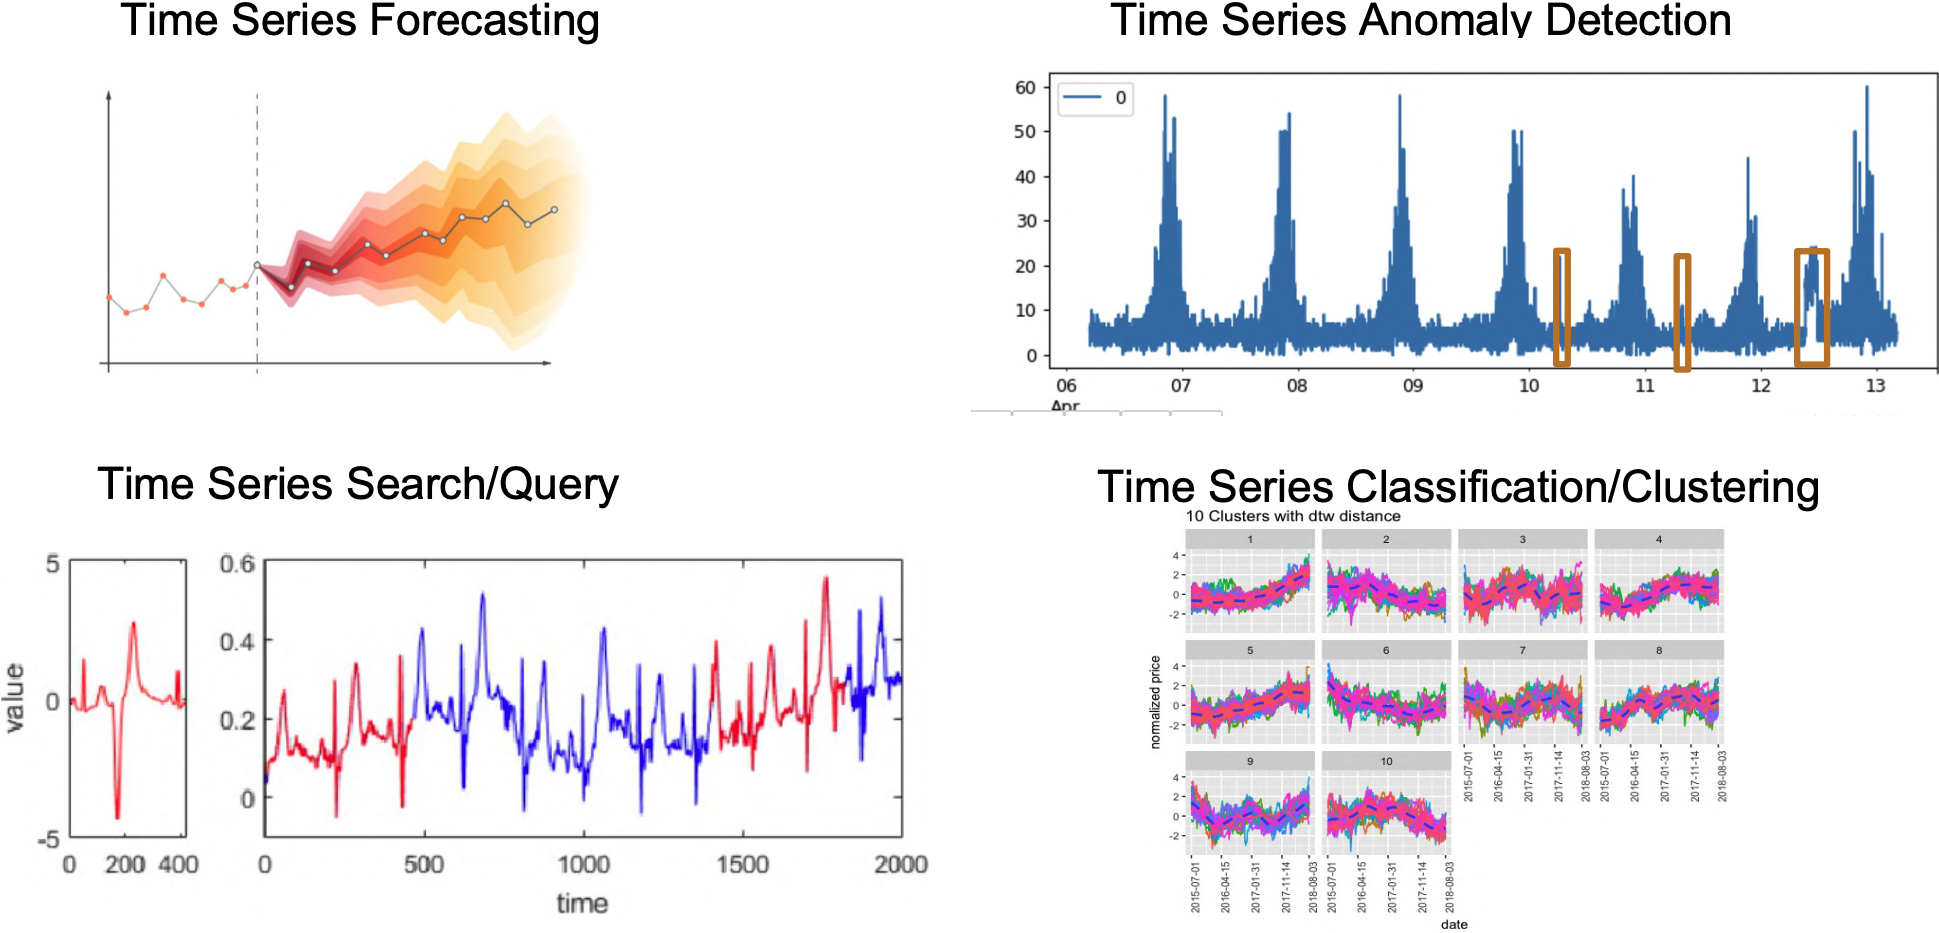
\includegraphics[width=\linewidth]{time_series_applications}
		\tiny{Image courtesy of \cite{wen2022robust}.}
	\end{figure}
\end{frame}

\begin{frame}
	\frametitle{From Forecast to Decision}
	\begin{itemize}
		\item Allocate resource based on demand forecast
		\item Peak demand vs. average demand
		\item Lead time and forecast horizon
	\end{itemize}
	\vfill
	\begin{figure}
		\centering
		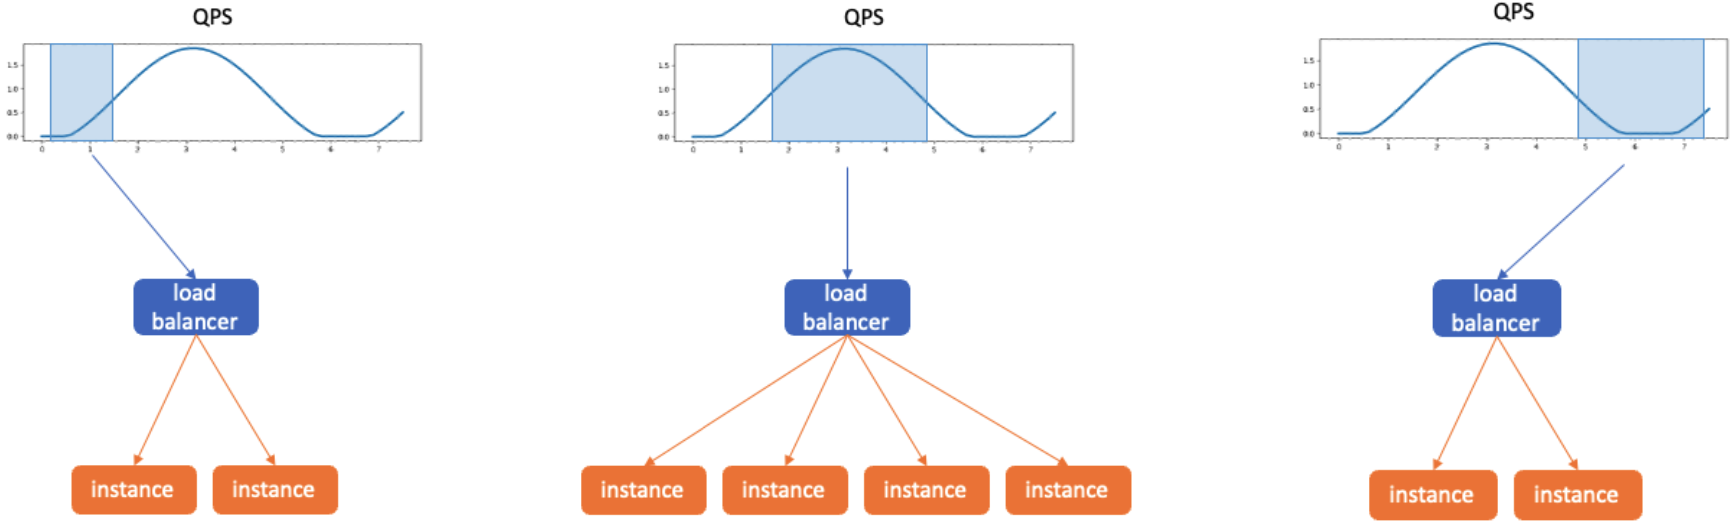
\includegraphics[width=\linewidth]{forecast}
		\tiny{Image courtesy of \cite{wen2022robust}.}
	\end{figure}
\end{frame}

\begin{frame}
	\frametitle{From Anomaly Detection to Cause Analysis}
	\begin{columns}
		\begin{column}{0.4\linewidth}
			\begin{figure}
				\centering
				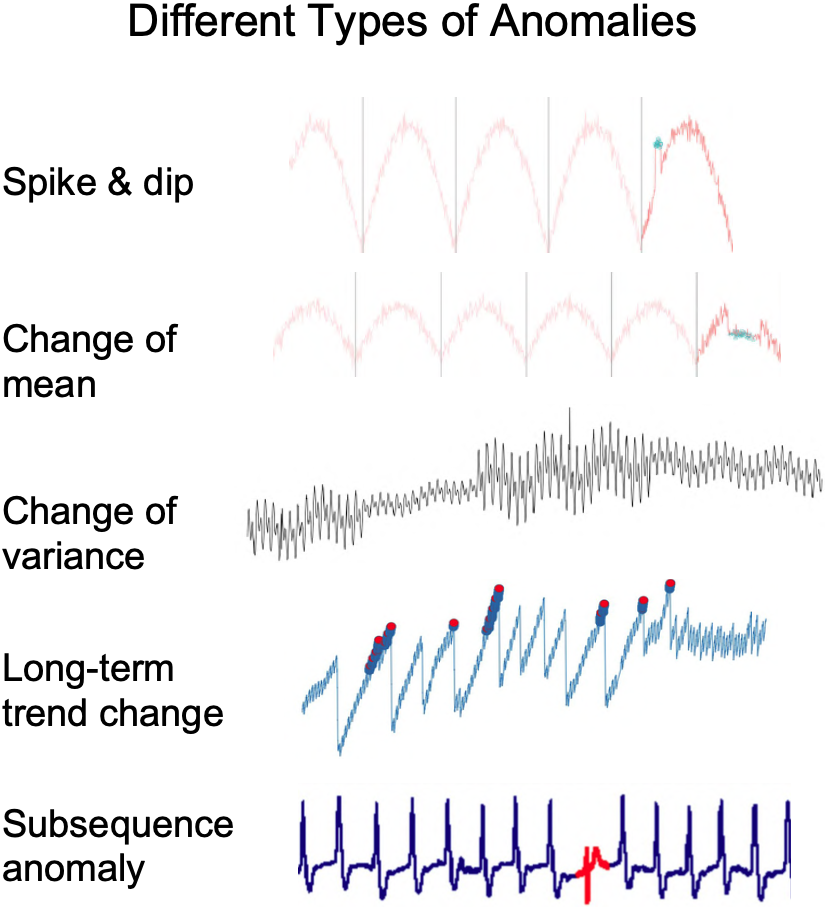
\includegraphics[width=\columnwidth]{anomaly}
			\end{figure}
		\end{column}
		\hfill
		\begin{column}{0.55\linewidth}
			\begin{itemize}
				\item<1> Time series is predictable since some of its properties are stable, e.g. WSS process
					\begin{itemize}
						\item Period
						\item Mean
						\item Variance
						\item Trend
						\item Distribution
					\end{itemize}
				\item<1> Anomaly are the portion of the signal that breaks the previous pattern
				\item<2> Detection of anomaly is only the first step, the key is the root cause of the anomaly
				\item<2> Cause analysis leads to new understanding and improved procedure
			\end{itemize}
		\end{column}
	\end{columns}
\end{frame}

%-------------------------------------------------------------------------------

\subsection{Values in time series}
\begin{frame}
	\frametitle{Why Time Series (Data Science) Matters?}
	\large
	\begin{itemize}
		\item<1> Data science starts from understanding of observations of physical world / human behaviors
		\vspace{2mm}
		\item<1> The impact of changes due to the improved understanding is the value of the data science
			\begin{itemize}
				\item Improved understanding 
				\item Make decision and change procedures
				\item Change future world and behaviors
			\end{itemize}
		\vspace{2mm}
		\item<2> Artificial intelligence in data science is a approach to realize impact
				\begin{minipage}{0.48\linewidth}
					\begin{itemize}
						\item signal processing
						\item statistical analysis
					\end{itemize}
				\end{minipage}
				\hfill
				\begin{minipage}{0.5\linewidth}
					\begin{itemize}
						\item machine learning
						\item deep learning
					\end{itemize}
				\end{minipage}
		\vspace{2mm}
		\item<3> Only measurble impact is valued in corporative scenario
			\begin{itemize}
				\item Indivual evaluation: bonus, reward, and promotion
				\item Team growth: budget, resource, exposure
			\end{itemize}
	\end{itemize}
\end{frame}

%-------------------------------------------------------------------------------

\subsection{Methods for time series analysis}

\begin{frame}
	\frametitle{Data Preparation}
	\begin{columns}
		\begin{column}{0.7\linewidth}
			\begin{itemize}
				\item<1> Gathering data is the first (most important) step
					\begin{itemize}
						\only\item Garbage in, Garbage out 
						\item Data integrity, data completeness
					\end{itemize}
				\vspace{3mm}
				\item<2> Identify and collect the proper dataset
					\begin{itemize}
						\item Work with business stakeholder to collect data sources
						\item Collect, validate, and clean up the source tables
						\item Build a data pipeline and monitor for data drifting
					\end{itemize}
				\vspace{3mm}
				\item<3> Make the prepared data available
					\begin{itemize}
						\item Write an API or use existing data API (BigQuery, DeltaLake, etc.)
						\item Document the details of the dataset for data discovery
						\item Periodically review the quality of the source data
					\end{itemize}
			\end{itemize}
		\end{column}
		\hfill
		\begin{column}{0.3\linewidth}
			\begin{figure}
				\centering
				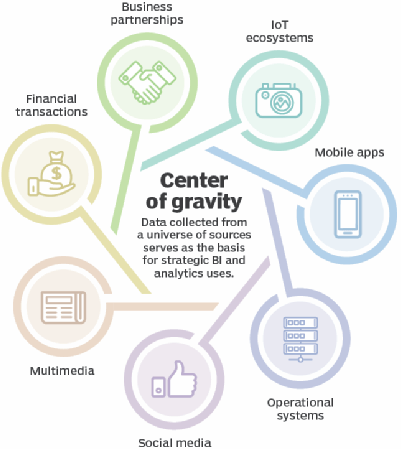
\includegraphics[width=\columnwidth]{data_collect}
			\end{figure}
		\end{column}
	\end{columns}
\end{frame}

\begin{frame}
	\frametitle{Feature Engineering}
	\begin{itemize}
		\item<1> Traditional Feature Engineering
			\begin{itemize}
				\item Summarized by experts with domain knowledge from small training sets
				\item Take advantage of years of experience and knowledges, e.g. spectral analysis: FFT
				\item Limited by our current understanding and observations
				\item More effective for complex system with a few dominant factors, e.g. long-term demand forecast
			\end{itemize}
		\item<2> Deep learning features (encoder-decoder architecture)
			\begin{itemize}
				\item Model learned from large amount of labeled data
				\item Open-ended data exploration guided by model structures
				\item Limited by volume of available labeled training data
				\item More effective for simple system with no obvious dominant factors, e.g. CV, NLP
			\end{itemize}
		\item<3> In reality, we have a mix of both in one complex system
			\begin{itemize}
				\item A heterogeneous learning system
				\item Connected machine intelligence of different small system (divide and conquer)
			\end{itemize}
	\end{itemize}
\end{frame}

\begin{frame}
	\frametitle{Modeling and Experiments}
	\begin{itemize}
		\item<1> Counter-intuitively, modeling is the least important part of enterprise pipelines
		\item<1> A collection of good enough off-the-shelf model to choose from
			\begin{itemize}
				\item Smoothing: Holt-Winters (\cite{winters1960forecasting}), Lewandowski model (JDA proprietary)
				\item Regression: ARIMA (\cite{ho1998use}), Prophet (\cite{taylor2018forecasting})
				\item Deep learning: Amazon DeepAR (\cite{salinas2020deepar}), Transformer, GNN
			\end{itemize}
			\vspace{3mm}
		\item<2> Focus on the use case and business value the model brings
			\begin{itemize}
				\item Model predicts at the right granularity the business use cases need
				\item Model has enough transparency required by the compliance 
					\begin{itemize}
						\item feature significance
						\item confidence intervals
					\end{itemize}
				\item Model training/inference can be completed in an efficient manner 
					\begin{itemize}
						\item Execution time
						\item Computation cost
					\end{itemize}
			\end{itemize}
	\end{itemize}
\end{frame}

\begin{frame}
	\frametitle{Data Visualization and Model Measurement}
	\begin{columns}
		\begin{column}{0.3\linewidth}
			\begin{itemize}
				\item Mark differences
					\vspace{5mm}
				\item Tell a story (ClubIQ)
					\vspace{5mm}
				\item Make an impact
					\vspace{5mm}
				\item Quantify success
					\vspace{5mm}
				\item Monitor metrics
			\end{itemize}
		\end{column}
		\hfill
		\begin{column}{0.7\linewidth}
			\begin{figure}
				\centering
				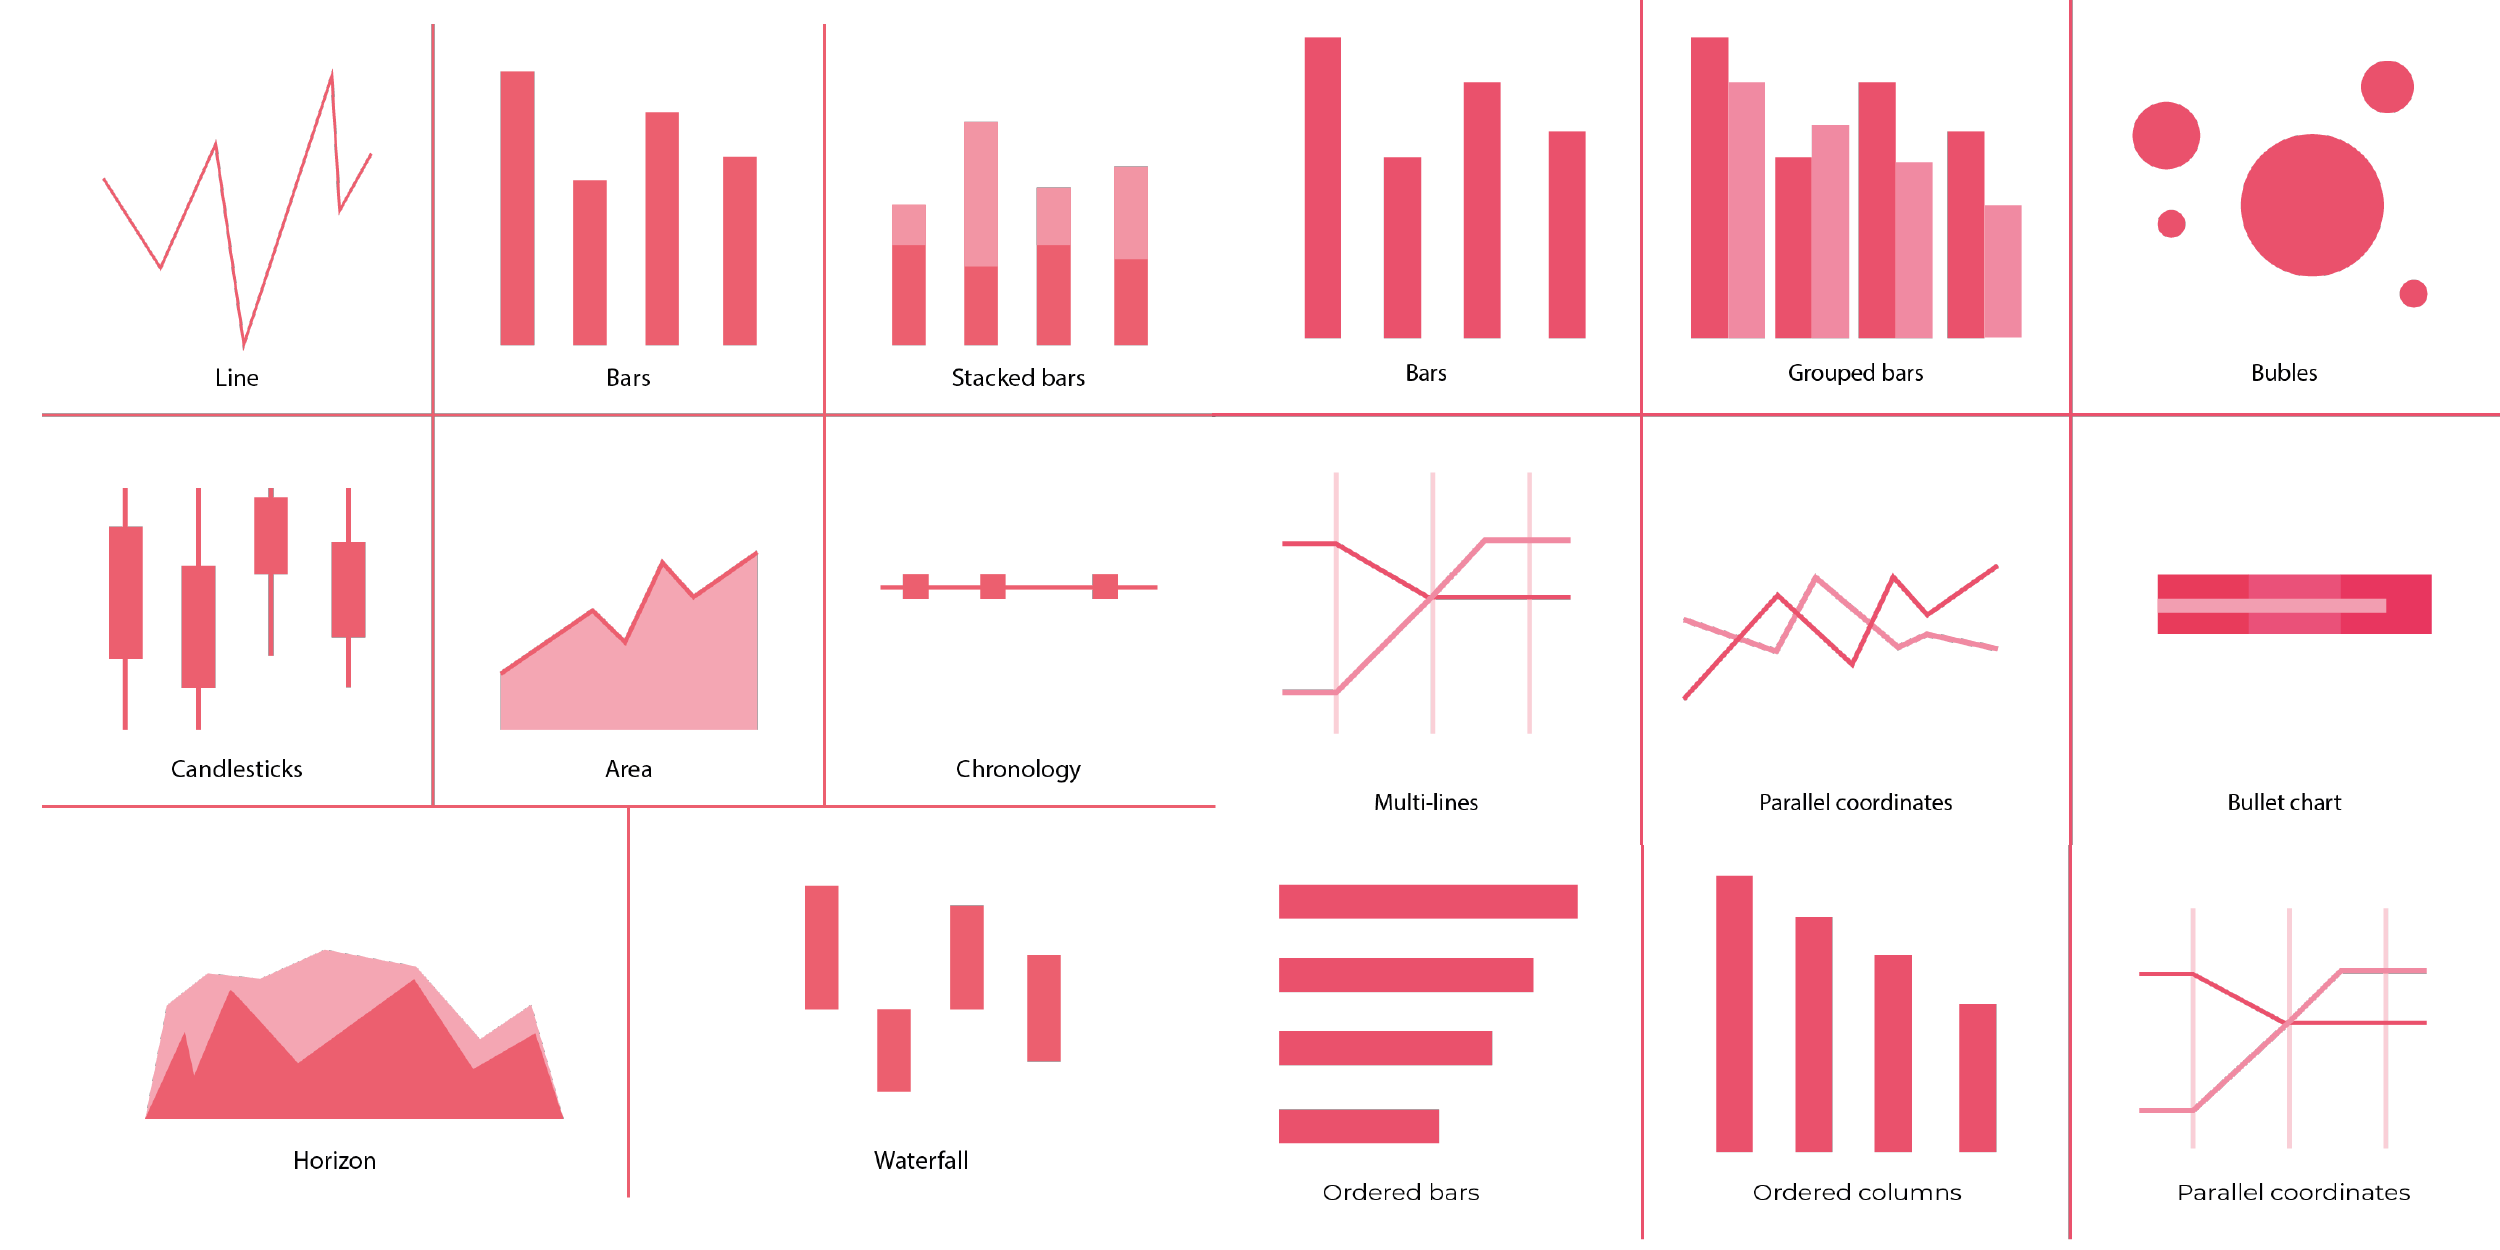
\includegraphics[width=\columnwidth]{data_visualization}
				\tiny \url{https://www.powerslide.io/en/blog/data-visualisation-what-you-need-to-know}
			\end{figure}
		\end{column}
	\end{columns}
\end{frame}


%-------------------------------------------------------------------------------
% Industry perspective for campus hires
%-------------------------------------------------------------------------------
\section{Industry perspective}
\subsection{Job market demands}
\begin{frame}
	\frametitle{Roles in my group}
	\begin{itemize}
		\item<1> Data Scientists (DS)
			\begin{itemize}
				\item Convert business problem to a data science problem
				\item Feature engineering, model design, system validation
				\item Visualization and communication to business partners
			\end{itemize}
		\item<2> Data Engineers (DE)
			\begin{itemize}
				\item Work with data stakeholder to collect and store data
				\item Clean up dataset and make it available for data science and engineering teams
				\item Build data pipeline to automate regular data update and monitor data drift
			\end{itemize}
		\item<3> Machine Learning Engineers (MLE)
			\begin{itemize}
				\item Build cloud/software infrastructures to support data science products
				\item Improve model effectiveness and efficiency (new models and tools)
				\item Maintain production ready system and long-term support of data science products
			\end{itemize}
		\item<4> Software Development Engineers (SDE)
			\begin{itemize}
				\item Work with business partner to define data science product
				\item Set requirements and acceptance criteria to data science and engineering teams
				\item Communicate data science and engineer teams' success and limitation
			\end{itemize}
	\end{itemize}
\end{frame}

\begin{frame}
	\frametitle{Other related roles}
	\begin{itemize}
		\item<1> Technical Product Managers (TPM)
			\begin{itemize}
				\item Work with business partner to define data science product
				\item Set requirements and acceptance criteria to data science and engineering teams
				\item Communicate data science and engineer teams' success and limitation
			\end{itemize}
			\vspace{5mm}
		\item<2> Data Analytics
			\begin{itemize}
				\item Conduct A/B tests to measure the effectiveness of data science product
				\item Visualization and reporting of efficiency analysis
			\end{itemize}
			\vspace{5mm}
		\item<3> UI/UX desginers
			\begin{itemize}
				\item Work with business team to identify the requirements for user interface
				\item Collaborate with data science team to provide necessary data for the interface
			\end{itemize}
	\end{itemize}
\end{frame}

\begin{frame}
	\frametitle{DS, MLE, and SDE}
	\begin{itemize}
		\item Owner of the product from end to end
			\begin{itemize}
				\item Help the product to define product and make measurement of success (PM)
				\item Design and implement data science models and pipeline (DS \& MLE)
				\item Assist in product delivery, maintenance, and update of the pipeline (DE \& SDE)
			\end{itemize}
		\item Driver of the product adoption
			\begin{itemize}
				\item Convey business value to business team (TPM)
				\item Measure impact of the product (DA)
			\end{itemize}
	\end{itemize}
	\vfill
	\begin{figure}
		\centering
		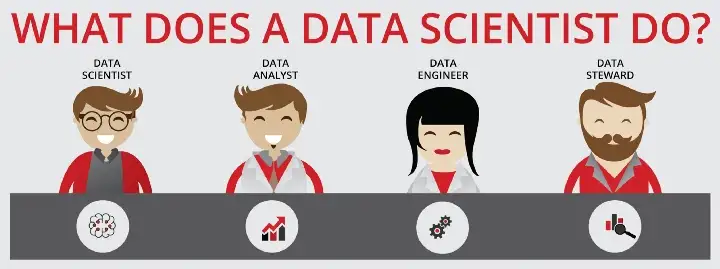
\includegraphics[width=0.8\linewidth]{data_scientist}
	\end{figure}
\end{frame}

\begin{frame}
	\frametitle{Data Engineers (DE)}
	\begin{itemize}
		\item Owner of the data pipeline infrastructures
			\begin{itemize}
				\item Implement and maintain data pipeline for batch or real-time access
				\item Monitor for potential data drift and data quality issues
			\end{itemize}
		\item Governer of the data access and compliance
			\begin{itemize}
				\item Grant and track access control of data source
				\item Meet government and company compliance for data access and usage
			\end{itemize}
	\end{itemize}
	\vfill
	\begin{figure}
		\centering
		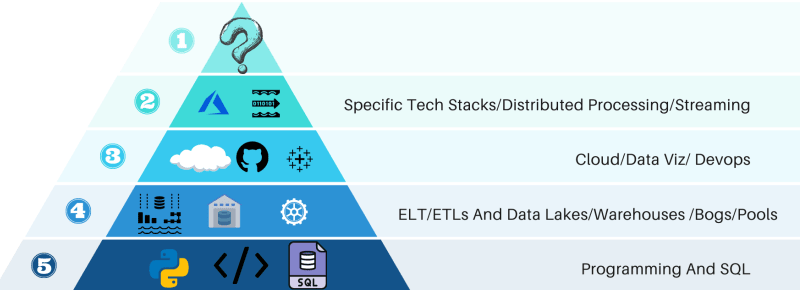
\includegraphics[width=0.8\linewidth]{data_engineer}
	\end{figure}
\end{frame}

%-------------------------------------------------------------------------------

\subsection{A product driving perspective}

\begin{frame}
	\frametitle{Product is your best Testimony}
	\begin{itemize}
		\item<1> Budget is granted on specific product but not technology
			\begin{itemize}
				\item Team is formed to ensure the success of a specific product
				\item People with background around similar technologies are put into a group
				\item End goal is for efficiency but not necessary technology advance
			\end{itemize}
			\vspace{5mm}
		\item<2> Success is measured via the business impact the products brings
			\begin{itemize}
				\item Understand what is the value your product brings to the team
				\item Quantify your measurement in unit of dollar when possible
			\end{itemize}
			\vspace{5mm}
		\item<3> Trade offs and hard decisions
			\begin{itemize}
				\item Re-privatization happens frequently
				\item Products with more business impact are bring to the front
			\end{itemize}
	\end{itemize}
\end{frame}

\begin{frame}
	\frametitle{Product is the driving force behind innovation}
	\begin{itemize}
		\item Product-centric vs. customer-centric
		\item Make a product that you are proud of
			\begin{itemize}
				\item Innovation is a by-product solving hard problems while making the product
				\item Stay connected with academia and on top of the latest breakthroughs
			\end{itemize}
	\end{itemize}
	\vfill
	\begin{figure}
		\centering
		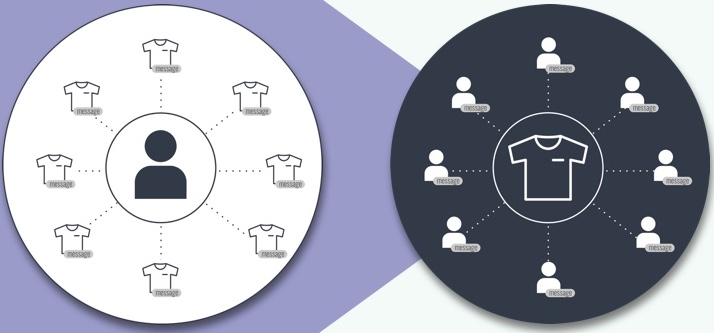
\includegraphics[width=0.7\linewidth]{product_customer}
	\end{figure}
\end{frame}

%-------------------------------------------------------------------------------

\subsection{A growth mindset}

\begin{frame}
	\frametitle{The Manager's Path (\cite{fournier2017manager})}
	\begin{columns}
		\begin{column}{0.7\linewidth}
			\begin{itemize}
				\item Explore your interests and establish your technical competence as an individual contributor
					\vspace{5mm}
				\item Advance and try out management as tech lead
				\item People Manager is not a promotion but a different job
					\vspace{5mm}
				\item Be the leader of innovation, technical or management
				\item Climb the tech ladder is interesting and rewarding
					\vspace{5mm}
				\item Don't be afraid of switching your career path to align with your passion
			\end{itemize}
		\end{column}
		\hfill
		\begin{column}{0.3\linewidth}
			\begin{figure}
				\centering
				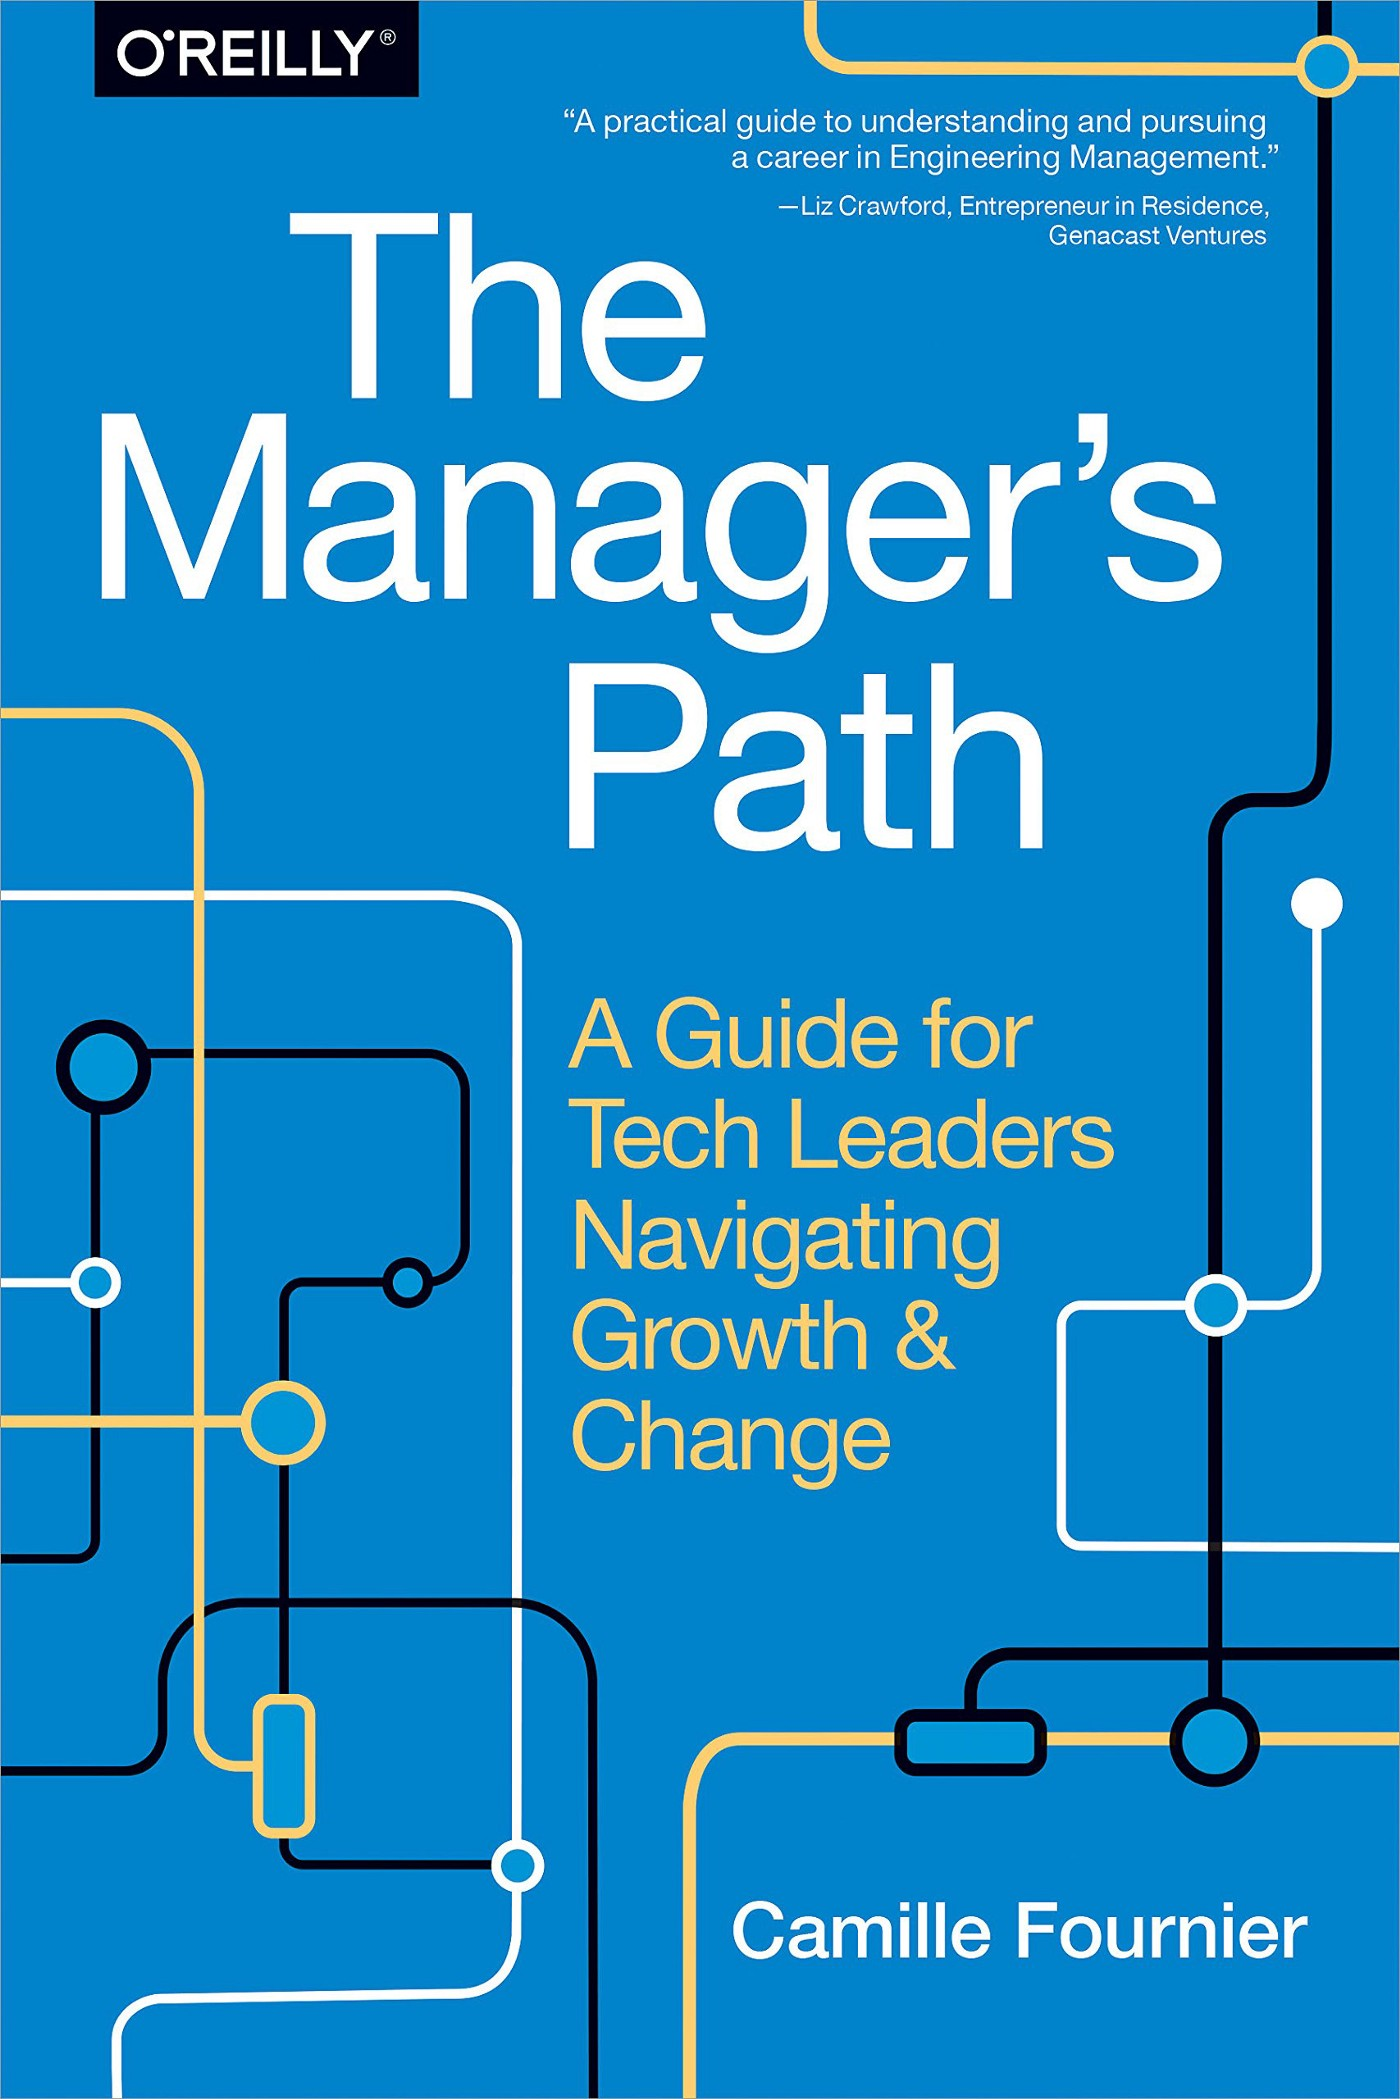
\includegraphics[width=\columnwidth]{manager}
			\end{figure}
		\end{column}
	\end{columns}
\end{frame}

\begin{frame}
	\frametitle{Zero to One (\cite{thiel2014zero})}
	\begin{columns}
		\begin{column}{0.7\linewidth}
			\begin{itemize}
				\item In the long run, innovation is the most important driving force behind economies
					\vspace{8mm}
				\item Today's best practice leads to dead ends
					\begin{itemize}
						\item You need to be different to be better (Bose)
						\item Fail and fail fast (MSR)
					\end{itemize}
					\vspace{8mm}
				\item Find values in unexpected places
					\begin{itemize}
						\item Thinking about first principles instead of formulas
						\item Nothing worth learning can be taught
					\end{itemize}
			\end{itemize}
		\end{column}
		\hfill
		\begin{column}{0.3\linewidth}
			\begin{figure}
				\centering
				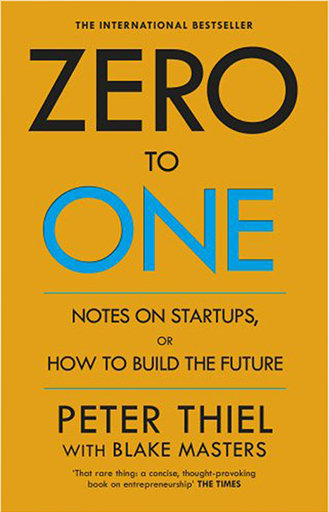
\includegraphics[width=\columnwidth]{zero}
			\end{figure}
		\end{column}
	\end{columns}
\end{frame}

\begin{frame}
	\frametitle{Reflection on recent macro economy changes}
	\begin{itemize}
		\item Cyclic nature of business, contraction follows expansion
			\begin{itemize}
				\item Industrial cycles, e.g. Oil and gas, semiconductor, agriculture
				\item Domestic and international market cycles
			\end{itemize}
		\item Growth happened in the downturn and harvested in the upturn (Amazon)
			\begin{itemize}
				\item Study and get a relevant degree for next upturn
				\item Gain experience and connections (my intern story)
				\item Pursue your own idea by starting a company
			\end{itemize}
	\end{itemize}
	\vfill
	\begin{figure}
		\centering
		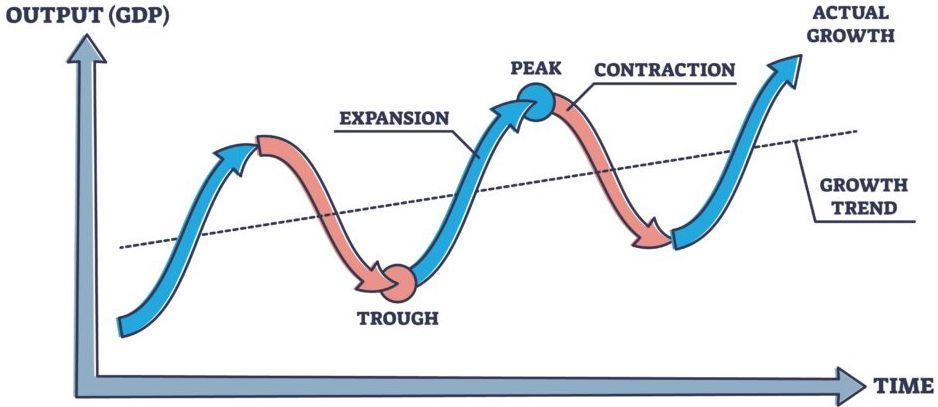
\includegraphics[width=0.6\linewidth]{business_cycles}
	\end{figure}
\end{frame}

%-------------------------------------------------------------------------------
% Summary
%-------------------------------------------------------------------------------

\begin{frame}
	\frametitle{Summary}
	\tableofcontents
\end{frame}

%-------------------------------------------------------------------------------
% Q & A
%-------------------------------------------------------------------------------
\begin{frame}
	\center
	\Huge Q \& A
\end{frame}

\begin{frame}[t,allowframebreaks]
	\frametitle{References}
	\tiny
	\printbibliography
\end{frame}

\end{document}
